% !TEX root = ../main.tex

%************************************************
\chapter{Introduction}
\label{ch:intro}
%************************************************

\section{The discovery of quasars}

In $1963$, the powerful radio source $3$C $273$ was identified as a star-like, thirteenth magnitude object with a strongly redshifted\footnote{Redshift $z=c(\Delta \lambda/\lambda)=0.158$, where $c$ is the speed of light.} optical spectrum \citep{schmidt63}. 
This finding implied $3$C $273$ was at an enormous distance (at least by the standards of the time). 
For an object this distant to appear so bright it must be extremely luminous: $10$ times more luminous, in fact, than the largest galaxies known. 
At the same time, its rapid variability meant that it could be no bigger than a light-week across.
$3$C $273$ was therefore a new kind of exotic object, at the edge of the known Universe.   
Understandably, its discovery caused a lot of excitement, both for astronomers and the wider public.
It was quickly realised that `quasars'\footnote{The term `quasar' originated as a contraction of `quasi-stellar radio source', although $90$ per cent of quasars are now known to be radio-quiet.}, and other lower-luminosity classes of active galactic nuclei (AGN)\footnote{Throughout this thesis we use the terms `quasar' and `Active Galactic Nucleus (AGN)' interchangeably to describe active super-massive black holes, although the term quasar is generally reserved for the luminous ($L_{\text{Bol}} > 10^{12}L_{\odot}$) subset of AGN.}, are powered by the release of gravitational potential energy as mass is accreted onto a super-massive\footnote{Super-massive: $10^{6 - 9}$ M$_\odot$.} black hole (BH) at the centre of a galaxy \citep[e.g.][]{hoyle63,salpeter64,lynden-bell69,lynden-bell71}. 

\section{The AGN-host galaxy connection}

Beginning in the early $1990$s, inactive super-massive BHs were found in the centres of many nearby massive galaxies \citep[e.g.][]{kormendy95,ferrarese05,kormendy13}.
This proved that, rather than being rare and exceptional objects, quasar activity was in fact a stage in the life of all massive galaxies \citep[e.g.][]{lynden-bell69}. 
Shortly after, it was discovered that the BH mass was tightly correlated with properties of the host-galaxy bulge \citep[e.g. the stellar velocity dispersion, $\sigma$, which is proportional to the bulge mass; e.g.][]{magorrian98,ferrarese00,gebhardt00,graham01,tremaine02,marconi03,aller07,gultekin09}.
This was an unexpected finding, given that the sphere-of-influence\footnote{Sphere-of-influence: where the gravity of the BH dominates over the other mass components.} of a BH \citep[$\lesssim100$ parsecs; e.g.][]{kormendy13}, is many orders of magnitude smaller than the dimensions of a typical galactic bulge. 
The tight correlation between their masses suggested that the BH and the host-galaxy bulge grow synchronously.
Both the density of quasars and the cosmic star formation history evolve strongly with redshift and peak at $2 \lesssim z \lesssim 3$ \citep[e.g.][]{boyle98,brandt05,richards06b}. 
The similarity of their cosmic evolution was taken as further evidence for the existence of an intimate connection between quasars and their host galaxies. 

In a currently favoured model, rapid BH fuelling and star-formation are triggered by a gas-rich galaxy merger \citep[e.g.][]{hopkins06a}, satellite accretion or secular processes \citep[e.g.][]{fanidakis12}. 
The energetic output of the rapidly-accreting BH couples with the gas in the host-galaxy and regulates star formation and the growth of the BH itself \citep[e.g.][]{silk98,king03,dimatteo05,king15}. 
This process, which is referred to as `quasar feedback', is also commonly invoked to reproduce the high-mass end of the galaxy luminosity function in cosmological simulations \citep[e.g.][]{kauffmann00}.  
The insight that quasars may play a crucial role in the evolution of galaxies has led to an explosion of interest in their properties in recent years. 

\section{AGN: the current paradigm}

\begin{figure}
  \centering
  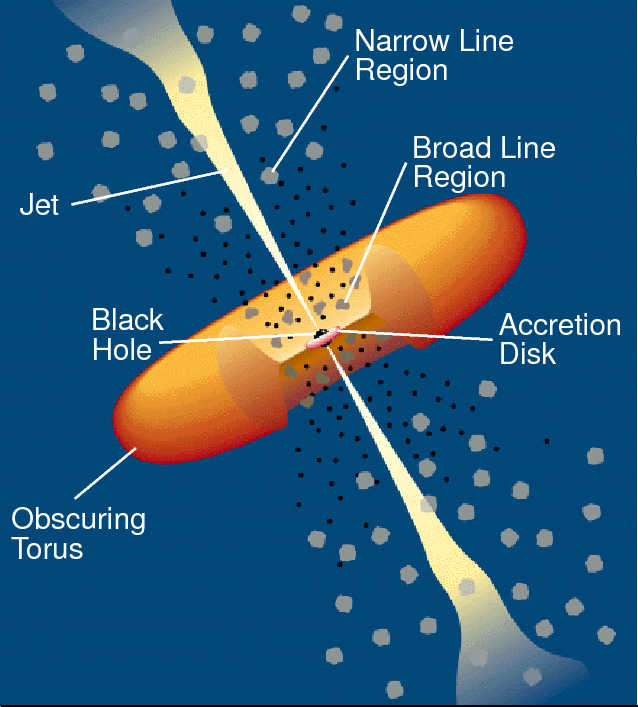
\includegraphics[width=0.5\textwidth]{figures/chapter05/urry_model}
  \caption[{Illustration of the physical structure of an AGN in a simple orientation-based unification model.}]{Cartoon picture of the inner regions on an AGN. Credit: \citet{urry95}.}
  \label{fig:agnmodel}
\end{figure}

The basic features of the current AGN paradigm are widely accepted, although many of the details are unknown. 
The basic features are: a hot accretion disc surrounding a super-massive BH, rapidly orbiting clouds of ionised gas, and a dusty, obscuring structure (generally referred to as the `torus'). 
Collimated jets of relativistic plasma and/or associated lobes are also seen in the $10$ per cent of quasars that are radio-loud \citep[e.g.][]{peterson97}. 
A cartoon picture illustrating the basic structure of an AGN is shown in Figure~\ref{fig:agnmodel}. 

\subsection{Accretion disc}

Material is pulled towards a super-massive BH and sheds angular momentum through viscous and turbulent processes in a hot accretion disc \citep[e.g.][]{begelman85}. 
The accretion disc reaches temperatures of $\sim10^6$ K, and radiates primarily at ultra-violet to soft-X-ray wavelengths. 

\subsection{Broad line region}

One of the pre-eminent features of many AGN spectra are broad optical and ultra-violet emission-lines produced in the broad line region (BLR). 
The BLR consists of gas clouds at distances from several light-days to several light-months that are photo-ionised by the ultra-violet continuum emission emanating from the accretion disc.  
Because of the close proximity to the central super-massive BH, bulk motions are dominated by gravity and radiation pressure from the accretion disc.
The very broad emission-line widths are assumed to be Doppler-broadened, and imply line-of-sight velocities of many thousands of \kms. 

Emission-line peak wavelengths can differ significantly \citep[e.g.][]{gaskell82}. 
Higher ionisation lines (including \ion{C}{IV}) are blueshifted relative to lower-ionisation lines (including \ion{MgII} and \hb), which are approximately at the AGN systemic redshift. 
This suggests that the structure of the BLR is stratified, with higher-ionisation lines emitted in regions where radial motions are significant.  

\subsection{Dusty torus}

Farther out from the central engine on parsec-scales are dusty, molecular clouds which are co-planar with the accretion disc. 
These dusty clouds are generally referred to as the `torus'. 
The torus is a central feature of orientation-based unification schemes \citep[e.g.][]{antonucci93} in which differing observational properties are explained as the effect of observing anisotropic objects in different orientations. 
In a Type II AGN, the system is observed in an edge-on configuration and, as a result, emission from the accretion disc and BLR is obscured by the dusty torus.
The orientation of a Type I AGN is such that the observer has direct sight-lines to the accretion disc and BLR. 
Although this simple picture (shown in Figure~\ref{fig:agnmodel} as well as in countless other publications) is a useful starting point, the idea of a torus as a static, doughnut-like structure is almost certainly a gross over-simplification. 
For example, the problem of maintaining the large scale height required to explain the observed fraction of Type I/II AGN has long been recognized \citep[e.g.][]{krolik88}. 
In one set of more realistic models, the torus is a dusty wind blown from the accretion disc \citep[e.g.][]{konigl94,everett09,gallagher12,everett05,keating12,elitzur06}. 

\subsection{Narrow line region}

Farther away from the central BH and beyond the dusty torus is the spatially-extended narrow emission-line region (NLR). 
Like the BLR, the NLR is ionised by radiation from the accretion disc. 
Unlike the BLR, densities in the NLR are low enough that forbidden transitions are not collisionally suppressed.
Because of its high equivalent width, [\ion{O}{III}]\l$5008$ is the most studied of the narrow quasar emission-lines.  
Emission-line widths are typically hundreds of \kms\, in the NLR.
The size of the NLR grows with the AGN luminosity, and can reach kilo-parsec scales in luminous quasars \citep[e.g.][]{hainline13}.    

\section[Large quasar surveys]{The advent of large surveys and the systematic study of AGN properties}

The Palomar-Green (PG) Bright Quasar Survey \citep[BQS;][]{schmidt83}, the first large-area quasar survey, identified $114$ quasars via their ultra-violet excess relative to stars. 
\citet{boroson92} were among the first to use the PG quasar sample to analyse quasar spectroscopic properties in a systematic way. 
In their landmark study, they used a principle component analysis (PCA) to identify the features responsible for the largest variance in quasar spectra. 
The first eigenvector of their PCA decomposition - generally referred to as `eigenvector 1' (EV$1$) - is correlated with the FWHM of the broad \hb emission-line and the relative strengths of optical \ion{Fe}{II} and \hbns. 
The underlying driver behind EV$1$ is thought to be the Eddington ratio\footnote{Eddington ratio: $L/L_{\text{Edd}}$, where the Eddington luminosity $L_{\text{Edd}}$ ($=3.2\times10^4(M/M_\odot)L_\odot$) is the maximum luminosity set by the balance of outward radiation pressure and inward gravitational force.}. 

With the advent of CCD\footnote{CCD: Charge coupled device.} technology came a new generation of optical spectroscopic surveys, most notably the Sloan Digital Sky Survey \citep[SDSS;][]{york00} and the $2$QZ survey \citep{croom04}. 
SDSS, and the next-generation SDSS-III: Baryon Oscillation Spectroscopic Survey \citep[BOSS;][]{dawson13}, now contain spectra of $\sim400\,000$ AGN and quasars. 
These large, uniform data sets have revolutionised the study of AGN and quasars by facilitating statistical studies of their properties covering wide ranges in redshift and luminosity.

Emission-lines provide a wealth of information about the properties of AGN and their environments. 
The rest-frame optical region in particular includes a number of strong emission features, including the Balmer lines and the [\ion{O}{III}] doublet that are used to measure BH masses, accretion rates, systemic redshifts and outflow properties. 
However, at $z\sim2$, rest-frame optical lines are redshifted to near-infrared wavelengths. 
Near-infrared spectroscopy is therefore essential for a complete understanding of quasars during the peak epoch of galaxy formation. 
Spectroscopic observations are challenging at infrared wavelengths, and there are far fewer infrared observations of quasars than optical ones. 
However, in Chapter~\ref{ch:nirsample}, we describe the construction of a near-infrared spectroscopic catalogue containing $462$ redshift $1.5 < z < 4$ quasars. 
This is the largest sample of its kind, and has facilitated investigations of quasar BH masses and outflow properties which are described in Chapters~\ref{ch:bhmass} and \ref{ch:nlr}.   

\section{Measuring black hole masses}

The BH mass is one of the most important physical parameters of a quasar and considerable resources have been devoted to measuring the masses of BHs in active galaxies. 
Large-scale studies of AGN and quasar demographics have become possible through the calibration of single-epoch virial-mass estimators using results from reverberation-mapping campaigns \citep[e.g.][]{peterson10,vestergaard11,marziani12,shen13}.  

\subsection{Reverberation mapping}

Under the assumptions that the BLR dynamics are virialised\footnote{The virial theorem states that the average kinetic energy of a system is equal to half of the average negative potential energy.} and the gravitational potential is dominated by the BH, the BH mass is given by:

\begingroup\makeatletter\def\f@size{11}\check@mathfonts
\begin{eqnarray}
M_{\text{BH}} \simeq \frac{V_{\text{Virial}}^2R_{\text{BLR}}}{G} 
\end{eqnarray}
\endgroup

\noindent where $V_{\text{virial}}$ is the virial velocity in the BLR and $R_{\text{BLR}}$ the characteristic BLR radius.
The problem of measuring the mass therefore reduces to the problem of measuring the velocity and orbital radius of the line-emitting clouds in the BLR. 

Continuum variability is a common characteristic of quasars, owing to the stochastic nature of the accretion process.  
Because the BLR is photo-ionized by the continuum, the broad emission-lines also vary with some characteristic lag, which is related to the light travel time across the BLR. 
The reverberation mapping method, first proposed by \citet{blandford82a}, uses the time lag between variations in the continuum emission and correlated variations in the broad line emission to measure the typical size of the BLR \citep[e.g.][]{peterson93,netzer97,peterson14}. 

The typical velocity in the BLR is measured from the Doppler-broadened width of an emission-line produced in the BLR. 
Since the structure and geometry of the BLR is unknown, a virial coefficient, $f$, is introduced to transform the observed line-of-sight velocity inferred from the line width into a virial velocity.
Unfortunately, $f$ is unknown and likely varies from object to object.  
In practice, the value of $f$ is empirically determined by requiring that the reverberation-mapping masses are consistent with those predicted from the $M_{\text{BH}}$-$\sigma$ relation for local inactive galaxies. 

Because reverberation mapping depends on temporal resolution rather than spatial resolution, this technique can be applied out to much greater distances than direct dynamical modelling \citep[e.g.][]{kormendy13}.
However, because reverberation mapping relies on dense spectrophotometric monitoring campaigns which span many years, the number of AGN with measured lags is limited to $\sim50$ AGN \citep[e.g.][]{kaspi00,peterson04,kaspi07,bentz09,denney10,barth11,grier12}. 
This sample is strongly biased to low luminosity Seyfert $1$ galaxies\footnote{Seyfert 1: A low-luminosity ($L_{\text{Bol}} < 10^{12}L_{\odot}$) class of AGN with broad emission-lines and clearly detectable host-galaxies.}, and the maximum redshift is just $z\sim0.3$. 
Comprehensive statistical studies of active BHs, particularly during the epoch of peak galaxy formation ($z\gtrsim2$), therefore require a different approach to measuring BH masses. 

\subsection{Single-epoch virial estimates}

Reverberation mapping campaigns have also revealed a tight relationship between the radius of the BLR and the quasar optical (or ultra-violet) luminosity \citep[the $R_{\text{BLR}}-L$ relation; e.g.][]{kaspi00,kaspi07}.
This relation provides a much less expensive method of measuring the BLR radius, and large-scale studies of AGN and quasar demographics \citep[e.g.][]{greene05b,vestergaard06,vestergaard09,shen11,shen12,trakhtenbrot12} have thus become possible through the calibration of single-epoch virial-mass estimators using the reverberation-mapping measurements \citep[e.g.][]{vestergaard02,mclure02,vestergaard06,mcgill08,wang09,rafiee11,park13}.

With single-epoch virial masses, the growth rate of massive BHs can be measured across cosmic time. 
This conveys important information about the accretion processes occurring in active BHs \citep[e.g.][]{kollmeier06} and is crucial in order to understand the processes responsible for establishing the $M_{\text{BH}}$-$\sigma$ relation \citep[e.g.][]{bennert11}.
Single-epoch virial estimates have been used to calculate BH masses in the highest redshift quasars \citep[e.g. a $10^9$\,M$_\odot$ BH in a redshift $z=7.1$ quasar;][]{mortlock11}. 
Recent claims of a BH with mass $10^{10}$\,M$_\odot$ in a redshift $z=6.3$ quasar \citep[when the Universe is less than $1$ Gyr old;][]{wu15} challenges our understanding of the accretion histories of supermassive BHs \citep[e.g.][]{willott03}. 

The uncertainties in reverberation mapped BH masses are estimated to be $\sim 0.4$\,dex \citep[e.g.][]{peterson10}, and the uncertainties in virial masses are similar \citep[e.g.][]{vestergaard06}.
However, the main concern and biggest unknown is the extension of the method to high redshifts. 
This requires that the relations calibrated for sub-Eddington BHs with $M_{\text{BH}}\sim10^7\,M_\odot$ are valid for BHs with masses up to $10^{10}\,M_\odot$ that are radiating near the Eddington luminosity. 
Furthermore, the vast majority of reverberation mapping measurements are for \hb and so the $R_{\text{BLR}}-L$ relation that underpins the virial method has only been established using this line.
\hb is redshift beyond the reach of optical spectrographs at redshifts $z \gtrsim 0.7$, and extending the method to higher redshifts requires the secondary-calibration of other low-ionization emission-lines such as \ha and \ion{Mg}{II} \citep[e.g.][]{vestergaard02,mclure02,wu04,kollmeier06,onken08,wang09,rafiee11}.

At redshifts of $z\gtrsim 2$ the low-ionization hydrogen and \ion{Mg}{II} emission-lines are no longer present in the optical spectra of quasars and it is necessary to employ an emission-line in the rest-frame ultra-violet.  
The strong \ion{C}{IV} emission doublet is visible in the optical spectra of quasars to redshifts of $z\sim5$ and \ion{C}{IV}-derived BH masses have become the standard \citep[e.g.][]{vestergaard06,park13}.
However, \ion{C}{IV} has long been known to exhibit significant displacements to the blue and these `blueshifts' almost certainly signal the presence of strong outflows.
As a consequence, single-epoch virial BH mass estimates derived from \ion{C}{IV} velocity-widths are known to be systematically biased compared to masses from the hydrogen Balmer lines. 

In Chapter~\ref{ch:bhmass}, we use a sample of $230$ high-luminosity ($L_{\text{Bol}} = 10^{45.5}-10^{48}$ erg s$^{-1}$), redshift $1.5 < z < 4.0$ quasars with both \ion{C}{IV} and Balmer line spectra to quantify the bias in \ion{C}{IV} BH masses as a function of the \ion{C}{IV} blueshift. 
\ion{C}{IV} BH masses are shown to be a factor of five larger than the corresponding Balmer-line masses at \ion{C}{IV} blueshifts of $3000$\,\kms\, and are over-estimated by almost an order of magnitude at the most extreme blueshifts, $\gtrsim 5000$\,\kms.
Using the monotonically increasing relationship between the \ion{C}{IV} blueshift and the mass ratio BH(\ion{C}{IV})/BH(\hans), we derive an empirical correction to all \ion{C}{IV} BH masses.
The scatter between the corrected \ion{C}{IV} masses and the Balmer masses is $0.24$\,dex at low \ion{C}{IV} blueshifts ($\sim0$\,\kms) and just $0.10$\,dex at high blueshifts ($\sim3000$\,\kms), compared to $0.40$\,dex before the correction. 
The correction depends only on the \ion{C}{IV} line properties - i.e. the full-width at half-maximum (FWHM) and blueshift - and can therefore be applied to all quasars where \ion{C}{IV} emission-line properties have been measured, enabling the derivation of un-biased virial BH mass estimates for the majority of high-luminosity, high-redshift, spectroscopically confirmed quasars in the literature.

\section{Winds and outflows in AGN}
\label{sec:ch1-winds}

Quasars are very powerful sources of radiation, and are embedded in matter-rich environments at the centres of galaxies.
Strong winds, driven by some combination of gas pressure, radiation pressure, and magnetic forces, are to be expected under these conditions \citep[e.g.][]{blandford82b,proga00,everett05}. 
In line with these expectations, evidence for outflowing gas is common in the spectra of quasars. 

Perhaps the most dramatic evidence for outflows is seen in broad absorption-line quasars \citep[BAL quasars;][]{weymann91}.
BAL quasars are characterised by broad absorption features in the ultra-violet resonance lines of highly ionised \ion{N}{V}, \ion{C}{IV} and \ion{Si}{IV}. 
The absorption troughs are thousands of \kms\, wide and significantly blueshifted relative to the quasar rest-frame\footnote{Much rarer cases of redshifted BAL troughs do also exist \citep[e.g.][]{hall13}.}. 
The absorption is thought to occur in outflows reaching $60\,000$\,\kms\, \citep[e.g.][]{turnshek88}. 
The near-universal blueshifting of the observed absorption features can be understood if the far-side of the outflow is obscured by the accretion disc, and so only the near-side, which is moving towards the observer, is detected. 
The observed \ion{C}{IV} BAL fraction in radio-quiet quasars is $\sim15$ per cent \citep[e.g.][]{hewett03,reichard03}.
Outflows can also explain narrow ultra-violet and X-ray absorption-lines (NALs) which are seen in $\sim60$ per cent of Seyfert 1 galaxies \citep{crenshaw99} and some quasars \citep[e.g.][]{hamann97}. 
The blueshifting of high-ionisation lines in the BLR (including \ion{C}{IV}) can also be understood if the lines are produced in outflowing clouds (although see, e.g., \citealt{gaskell16}, for an alternative explanation). 
The blueshifting of \ion{C}{IV} appears to be nearly ubiquitous in the quasar population \citep[e.g.][]{richards02,richards11}. 

Together, these results suggest that outflows are very common and the energy released by quasars can have a dramatic effect on their immediate surroundings. 
Accretion-disc wind models have been developed to explain the wide range of emission and absorption-line phenomena which are observed \citep[e.g.][]{murray95,elvis00,proga00,everett05}.
  
In models for the co-evolution of quasars and galaxies, the energy released by quasars impacts galaxies on much larger scales than is probed by the emission and absorption diagnostics described above.  
In recent years, a huge amount of resources have been devoted to searching for observational evidence of galaxy-wide, quasar-driven outflows \citep[for recent reviews, see][]{alexander12,fabian12,heckman14}.
This has resulted in recent detections of outflows in AGN host-galaxies using tracers of atomic, molecular, and ionised gas with enough power to sweep their host-galaxies clear of gas \citep[e.g.][]{nesvadba06,arav08,nesvadba08,moe09,dunn10,alexander10,harrison12,harrison14,nesvadba10,rupke13,veilleux13,nardini15,feruglio10,alatalo11,cimatti13,cicone14}.  

The advent of large optical spectroscopic surveys (e.g. SDSS) has facilitated studies of the NLR in tens of thousands of AGN at redshifts $z\lesssim0.4$ which has provided constraints on the prevalence and drivers of ionised outflows \citep[e.g.][]{mullaney13,zakamska14}. 
Because of its high EQW, [\ion{O}{III}] is the most studied of the narrow AGN emission-lines.  
By following [\ion{O}{III}] to near-infrared wavelengths, we are able to extend these investigations to the redshift range when star formation and BH accretion peaked. 
In Chapter~\ref{ch:nlr}, we analyse the [\ion{O}{III}] properties of a sample of $354$ high-luminosity, redshift $1.5 < z < 4$ quasars. 
To date, this is the largest study of the NLR properties of high redshift quasars. 

Comparing our sample to SDSS AGN at lower redshifts and luminosities, we find [\ion{O}{III}] to be significantly broader, more blue-asymmetric and weaker. 
The [\ion{O}{III}] EQW is tightly correlated with the \ion{C}{IV} blueshift, and we propose that the NLR gas is being swept away on relatively short time-scales by quasar-driven outflows.
In quasars for which [\ion{O}{III}] is detected, we find that the blueshifting of [\ion{O}{III}] and \ion{C}{IV} are correlated. 
This establishes a connection between quasar-driven outflows in the broad and narrow line regions.  
We confirm earlier results that the EV$1$ correlations found in low-luminosity AGN also exist in high-redshift quasars and demonstrate that Independent Component Analysis (ICA) can be used to extend these results to spectra with lower signal-to-noise. 

\section{AGN spectral energy distributions}

\begin{figure}
  \centering
  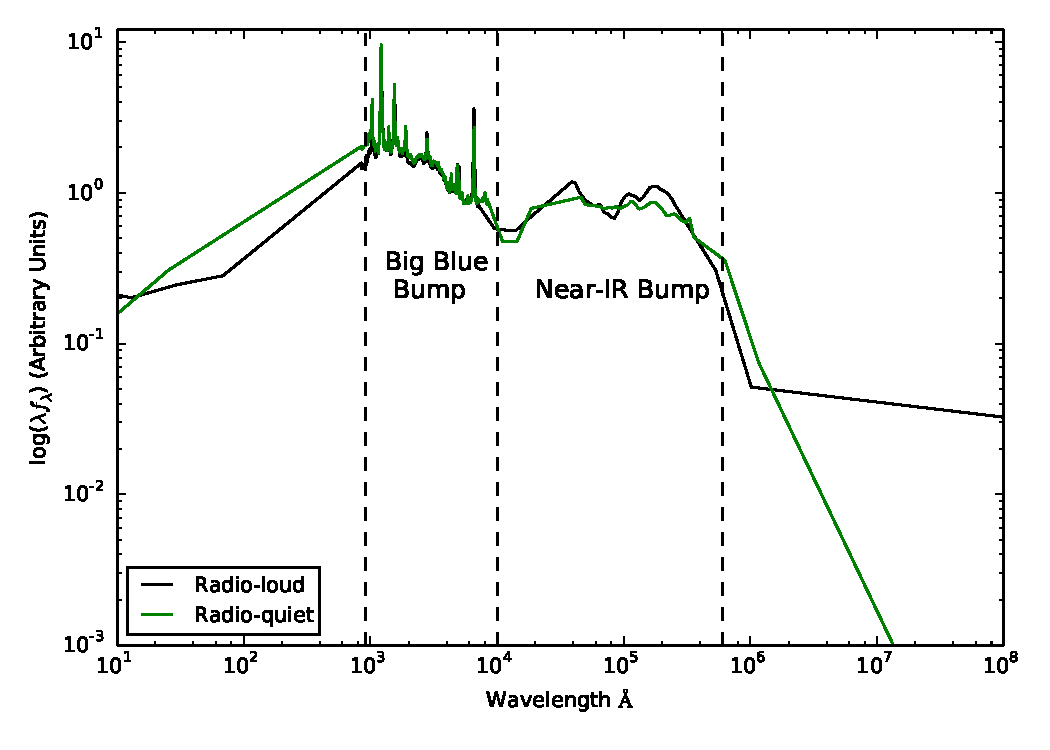
\includegraphics[width=\textwidth]{figures/chapter05/shangsed.pdf}
  \caption{Median radio-loud AGN SED from \citet{shang11}.}
  \label{fig:seyfert_sed}
\end{figure}

AGN emit strongly over many decades of the electromagnetic spectrum (Figure~\ref{fig:seyfert_sed}). 
Different physical processes dominate AGN spectral energy distributions (SEDs) at different frequencies. 
Hard X-ray emission is dominated by Compton up-scattering of accretion disk photons by electrons in a hot corona \citep[e.g.][]{sunyaev80}, ultra-violet/optical by thermal accretion disc emission, IR by dust at a wide range of temperatures, and radio by synchrotron emission in relativistic jets.   
A complete understanding of AGN properties therefore critically depends on the availability of multi-wavelength data that spans the full SED. 
Progress has been made in recent years using data from new sensitive, wide-field photometric surveys \citep[e.g.][]{roseboom13}. 
These surveys include the ultra-violet/optical SDSS, the near-infrared UKIRT Infrared Deep Sky Survey \citep[UKIDSS;][]{lawrence07} and the mid-infrared Wide-field Infrared Explorer \citep[WISE;][]{wright10}. 

To first order, AGN have remarkably similar SEDs that show very little dependence on luminosity, redshift, BH mass or accretion rate \citep[e.g.][]{elvis12,hao13}. 
In Chapter~\ref{ch:sed}, we build a simple parametric SED model that is able to reproduce the median optical-infrared colours of tens of thousands of SDSS AGN at redshifts $1<z<3$. 
On the other hand, the SED properties of individual quasars do show significant variation.
In particular, we find the spread at $1-2$ $\mu$m is large and suggests the presence of significant diversity in hot dust properties.
We find that the amount of hot dust is strongly correlated with the strength of outflows in the quasar BLR (parametrised using the \ion{C}{IV} blueshift) and consider the implications of this result in the context of accretion disc wind models \citep[e.g.][]{elitzur06}.
We demonstrate that apparent correlations between the hot dust abundance and BH mass and Eddington ratio result from systematic biases in the \ion{C}{IV}-based BH masses and disappear when new, unbiased BH mass estimates (derived in Chapter~\ref{ch:bhmass}) are adopted. 

\section{Note on adopted conventions}

Throughout this thesis, we adopt a $\Lambda$CDM cosmology with $h_0=0.71$, $\Omega_M=0.27$, and $\Omega_\Lambda=0.73$. 
All wavelengths and EQW measurements are given in the quasar rest-frame, and all emission-line wavelengths are given as measured in vacuum.
Unless otherwise stated, optical (i.e. SDSS) magnitudes are given in the AB system and infrared magnitudes in the Vega system, following the conventions of the original surveys. 



\section{Outline of thesis}

\todoinline{Include this?} 

